%% Based on a TeXnicCenter-Template by Gyorgy SZEIDL.
%%%%%%%%%%%%%%%%%%%%%%%%%%%%%%%%%%%%%%%%%%%%%%%%%%%%%%%%%%%%%

%------------------------------------------------------------
%
\documentclass{article}%
%Options -- Point size:  10pt (default), 11pt, 12pt
%        -- Paper size:  letterpaper (default), a4paper, a5paper, b5paper
%                        legalpaper, executivepaper
%        -- Orientation  (portrait is the default)
%                        landscape
%        -- Print size:  oneside (default), twoside
%        -- Quality      final(default), draft
%        -- Title page   notitlepage, titlepage(default)
%        -- Columns      onecolumn(default), twocolumn
%        -- Equation numbering (equation numbers on the right is the default)
%                        leqno
%        -- Displayed equations (centered is the default)
%                        fleqn (equations start at the same distance from the right side)
%        -- Open bibliography style (closed is the default)
%                        openbib
% For instance the command
%           \documentclass[a4paper,12pt,leqno]{article}
% ensures that the paper size is a4, the fonts are typeset at the size 12p
% and the equation numbers are on the left side
%
\usepackage{amsmath}%
\usepackage{amsfonts}%
\usepackage{amssymb}%
\usepackage{graphicx}%
\usepackage{epstopdf}

\addtolength{\textheight}{1.6cm}
\addtolength{\textwidth}{0.6cm}
\addtolength{\marginparwidth}{-1.2cm}
\addtolength{\headheight}{-2.1cm}

%-------------------------------------------
\newtheorem{theorem}{Theorem}
\newtheorem{acknowledgement}[theorem]{Acknowledgement}
\newtheorem{algorithm}[theorem]{Algorithm}
\newtheorem{axiom}[theorem]{Axiom}
\newtheorem{case}[theorem]{Case}
\newtheorem{claim}[theorem]{Claim}
\newtheorem{conclusion}[theorem]{Conclusion}
\newtheorem{condition}[theorem]{Condition}
\newtheorem{conjecture}[theorem]{Conjecture}
\newtheorem{corollary}[theorem]{Corollary}
\newtheorem{criterion}[theorem]{Criterion}
\newtheorem{definition}[theorem]{Definition}
\newtheorem{example}[theorem]{Example}
\newtheorem{exercise}[theorem]{Exercise}
\newtheorem{lemma}[theorem]{Lemma}
\newtheorem{notation}[theorem]{Notation}
\newtheorem{problem}[theorem]{Problem}
\newtheorem{proposition}[theorem]{Proposition}
\newtheorem{remark}[theorem]{Remark}
\newtheorem{solution}[theorem]{Solution}
\newtheorem{summary}[theorem]{Summary}
\newenvironment{proof}[1][Proof]{\textbf{#1.} }{\ \rule{0.5em}{0.5em}}

\begin{document}

\title{Department of  Statistics \\ STATS 784: Data Mining}
\author{Zhi Zhang, $\ $708439475, $\ $zzha822
\\The University of Auckland}
\date{August 16th, 2017}
\maketitle

%\begin{abstract}
%This is a sample document which shows the most important features of the Standard
%\LaTeX\ Journal Article class.
%\end{abstract}

\section{Question 1}
I use the data from "Boston" of library of MASS in R as the input data for the neural network I make myself. \\
\indent And the $\beta_{h}, \sigma$ function and $\alpha_{ih} (i \in {0, 1, 2, \cdots, n})$ are the random numeric generated by R function.\\
\indent The first process is to do data transformations for individual predictors, which including centering, scaling, and resolving distributional skewness. Centering and scaling are generally used to improve the numerical stability of some calculations. And after skewness transformation, the distribution is not entirely symmetric but these data are better behaved than when they were in the natural units.\\
\indent Another pre-process is to do data transformations for multiple predictors, using methods to resolve outliers and reduce the dimension of the data. Usually we an identify the outliers on a figure and there are some predictive models resistant to outliers. Data reduction techniques are another class of predictor transformations. These methods reduce the data by generating a smaller set of predictors that seek to capture a majority of the information in the original variables.\\
\indent Dealing with Missing Values is also important for pre-processing data. It is important to understand why the values are missing. First and foremost,
it is important to know if the pattern of missing data is related to the outcome. Missing data can be imputed and imputation has been extensively studied in the statistical literature. One popular technique for imputation is a K-nearest neighbor model. A new sample is imputed by finding the samples in the training set “closest” to it and averages these nearby points to fill in the value.\\
\indent Removing predictors is also used to get potential advantages for the data modeling. A rule of thumb for detecting near-zero variance predictors is:\\
\indent $\bullet$ The fraction of unique values over the sample size is low (say 10\%).\\
\indent $\bullet$ The ratio of the frequency of the most prevalent value to the frequency of the second most prevalent value is large (say around 20).\\
\indent In addition, collinearity is the technical term for the situation where a pair of predictor variables have a substantial correlation with each other. It is also
possible to have relationships between multiple predictors at once (called multicollinearity).
\indent Also adding predictors and binning predictors are also general techniques we used for pre-processing data before modeling. More details are discussing with the case of Cell Segmentation.

\subsection{Application2}
In "Applied Predictive Modelling" (Kuhn, M. and Johnson, K. (2013).), chapter 12, there is a case that decribes the application of Discriminant Analysis technology. \\
\indent Discriminant Analysis is one of the techniques of Classification Analysis for Data Mining. Generally it includes the techniques for linear and nonlinear classification models. In this chapter, the case is about Predicting Successful Grant Applications. The data of these applications are from a 2011 Kaggle competition sponsored by the University of Melbourne where there was interest in predicting whether or not a grant application would be accepted. In addition to predicting grant success, the university sought to understand factors that were important in predicting success.\\
\indent Logistic regression is a very popular model due to its simplicity and ability to make inferential statements about model terms. It is linear in the parameters, and these parameters are obtained by minimizing the sum of the squared residuals. It turns out that the model that minimizes the sum of the squared residuals also produces maximum likelihood estimates of the parameters when it is reasonable to assume that the model residuals follow a normal (i.e., Gaussian) distribution. \\
\indent Another important technique is called Linear Discriminant Analysis (LDA). This method define a linear discriminant function (may find an optimal discriminant vector) to do analysis and estimation. Examining the coefficients of the linear discriminant function can provide an understanding of the relative importance of predictors. Due to the inherent problem with LDA, as well as its other fundamental requirements, it is recommended that LDA be used on data sets that have at least 5–10 times more samples than predictors.\\
\indent The third technique is called Partial Least Squares Discriminant Analysis (PLSDA). For retrospectively or prospectively, measured predictors for any particular problem can be highly correlated or can exceed the number of samples collected. If either of these conditions is true, then the usual LDA approach cannot be directly used to find the optimal discriminant function. So we use PLS for the purpose of discrimination. Applying PLS in the classification setting with a multivariate response has strong mathematical connections to both canonical correlation analysis and LDA.\\
\indent In addition, Many classification models utilize penalties (or regularization) to improve the fit to the data, such as the lasso. And penalization strategies can be applied to LDA models. The penalized LDA model was applied to the grant data. The software for this model allows the user to specify the number of retained predictors as a tuning parameter. As the penalty increases and predictors are eliminated, performance improves and remains relatively constant until
important factors are removed. At this point, performance falls dramatically. As a result of the tuning process, six predictors were used in the model which is competitive to other models.\\
\indent The nearest-shrunken centroid model (also known as PAM, for predictive analysis for microarrays) is a linear classification model that is well suited for high-dimensional problems. The nearest shrunken centroid method has one tuning parameter: shrinkage. This model works well for problems with a large number of predictors since it has built-in feature selection that is controlled by the shrinkage tuning parameter. Nearest shrunken centroids were originally developed for RNA profiling data, where the number of predictors is large (in the many thousands) and the number of samples is small.

%\noindent The front matter has various entries such as\\
%\hspace*{\fill}\verb" \title", \verb"\author", \verb"\date", and
%\verb"\thanks"\hspace*{\fill}\\
%You should replace their arguments with your own.
%
%This text is the body of your article. You may delete everything between the commands\\
%\hspace*{\fill} \verb"\begin{document}" \ldots \verb"\end{document}"
%\hspace*{\fill}\\in this file to start with a blank document.


\section{Question 2}
First we load the Housing Price data from the URL and change variables \emph{\textbf{view}}, and \emph{\textbf{waterf}} to be used as factors for R functions.
\begin{verbatim}
> URL = "https://www.stat.auckland.ac.nz/~lee/784/Assignments/kc_house_data.csv"
> input.df = read.csv(URL)
> names(input.df) = c("id", "date", "price", "bedrooms", "bathrooms",
+ "sqftlv", "sqftlot", "floors", "waterfr", "view",
+ "cond", "grade", "sqfta", "sqftb", "yrb", "yrr",
+ "zip", "lat", "long", "sqftlv15", "sqftlot15")
> head(input.df)
          id            date   price bedrooms bathrooms sqftlv sqftlot floors
1 7129300520 20141013T000000  221900        3      1.00   1180    5650      1
2 6414100192 20141209T000000  538000        3      2.25   2570    7242      2
3 5631500400 20150225T000000  180000        2      1.00    770   10000      1
4 2487200875 20141209T000000  604000        4      3.00   1960    5000      1
5 1954400510 20150218T000000  510000        3      2.00   1680    8080      1
6 7237550310 20140512T000000 1225000        4      4.50   5420  101930      1
  waterfr view cond grade sqfta sqftb  yrb  yrr   zip     lat     long
1       0    0    3     7  1180     0 1955    0 98178 47.5112 -122.257
2       0    0    3     7  2170   400 1951 1991 98125 47.7210 -122.319
3       0    0    3     6   770     0 1933    0 98028 47.7379 -122.233
4       0    0    5     7  1050   910 1965    0 98136 47.5208 -122.393
5       0    0    3     8  1680     0 1987    0 98074 47.6168 -122.045
6       0    0    3    11  3890  1530 2001    0 98053 47.6561 -122.005
  sqftlv15 sqftlot15
1     1340      5650
2     1690      7639
3     2720      8062
4     1360      5000
5     1800      7503
6     4760    101930
>
> input.df$waterfr = factor(input.df$waterfr)
> input.df$view = factor(input.df$view)
> str(input.df)
'data.frame':   21613 obs. of  21 variables:
 $ id       : num  7.13e+09 6.41e+09 5.63e+09 2.49e+09 1.95e+09 ...
 $ date     : Factor w/ 372 levels "20140502T000000",..: 165 221 291 221 
              284 11 57 252 340 306 ...
 $ price    : num  221900 538000 180000 604000 510000 ...
 $ bedrooms : int  3 3 2 4 3 4 3 3 3 3 ...
 $ bathrooms: num  1 2.25 1 3 2 4.5 2.25 1.5 1 2.5 ...
 $ sqftlv   : int  1180 2570 770 1960 1680 5420 1715 1060 1780 1890 ...
 $ sqftlot  : int  5650 7242 10000 5000 8080 101930 6819 9711 7470 6560 ...
 $ floors   : num  1 2 1 1 1 1 2 1 1 2 ...
 $ waterfr  : Factor w/ 2 levels "0","1": 1 1 1 1 1 1 1 1 1 1 ...
 $ view     : Factor w/ 5 levels "0","1","2","3",..: 1 1 1 1 1 1 1 1 1 1 ...
 $ cond     : int  3 3 3 5 3 3 3 3 3 3 ...
 $ grade    : int  7 7 6 7 8 11 7 7 7 7 ...
 $ sqfta    : int  1180 2170 770 1050 1680 3890 1715 1060 1050 1890 ...
 $ sqftb    : int  0 400 0 910 0 1530 0 0 730 0 ...
 $ yrb      : int  1955 1951 1933 1965 1987 2001 1995 1963 1960 2003 ...
 $ yrr      : int  0 1991 0 0 0 0 0 0 0 0 ...
 $ zip      : int  98178 98125 98028 98136 98074 98053 98003 98198 98146 98038 ...
 $ lat      : num  47.5 47.7 47.7 47.5 47.6 ...
 $ long     : num  -122 -122 -122 -122 -122 ...
 $ sqftlv15 : int  1340 1690 2720 1360 1800 4760 2238 1650 1780 2390 ...
 $ sqftlot15: int  5650 7639 8062 5000 7503 101930 6819 9711 8113 7570 ...
\end{verbatim}
Next we transform the target to make it more symmetric, using the Box-Cox transformation.
\begin{verbatim}
> library(caret)
> trans = BoxCoxTrans(input.df$price)
> trans
Box-Cox Transformation

21613 data points used to estimate Lambda

Input data summary:
   Min. 1st Qu.  Median    Mean 3rd Qu.    Max.
  75000  321950  450000  540088  645000 7700000

Largest/Smallest: 103
Sample Skewness: 4.02

Estimated Lambda: -0.2
With fudge factor, Lambda = 0 will be used for transformations

>
> transPrice = predict(trans, input.df$price)
> par(mfrow = c(1, 2))
> hist(input.df$price, main = "Untransformed", nclass = 30)
> hist(transPrice, main = "Transformed", nclass = 30)
\end{verbatim}
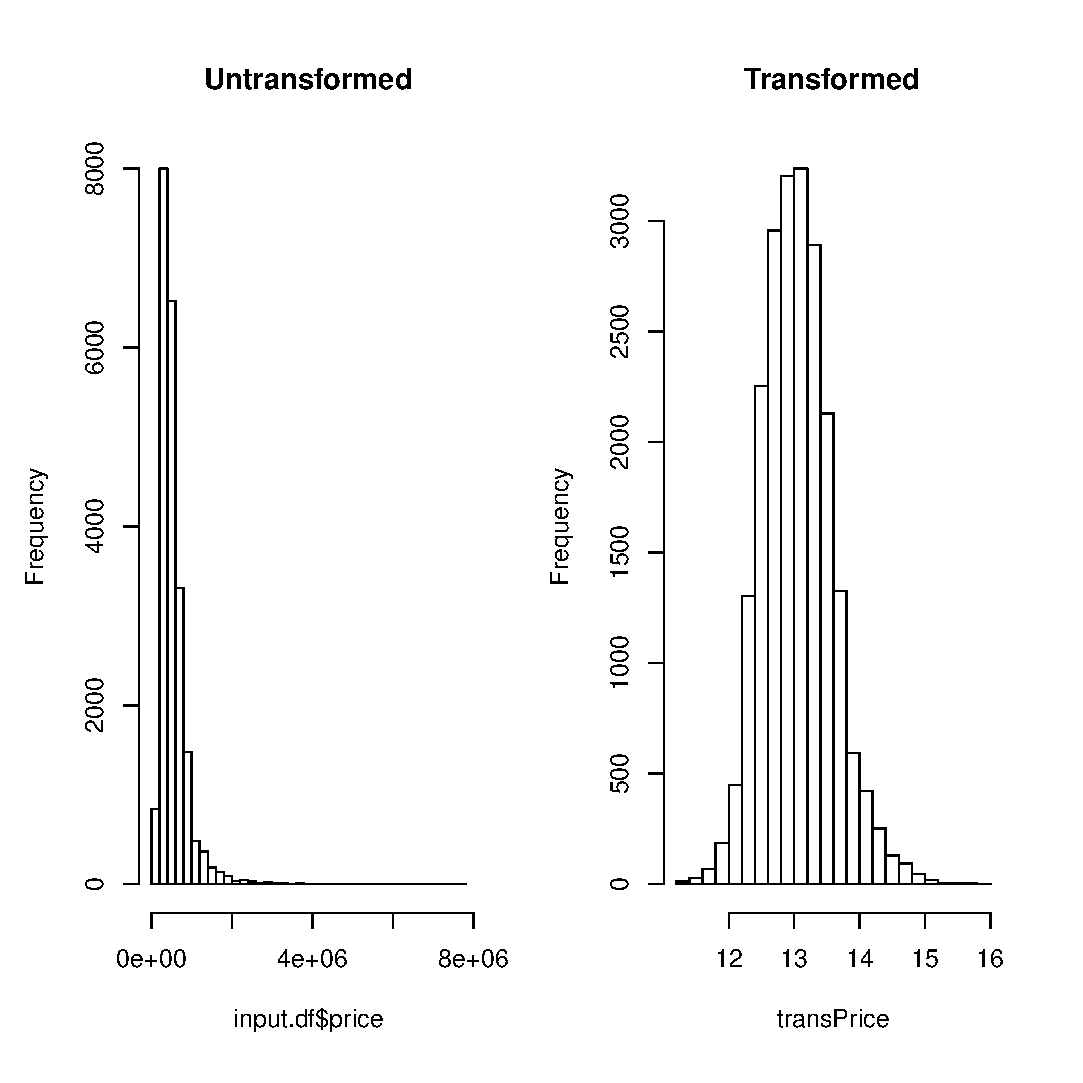
\includegraphics[width=\textwidth]{Symmetric.eps}
From the plot we see that the transformed data is more symmetric, which will get more adavantage to the prediction. We will use transformed  \emph{\textbf{price}} to do the prediction.
\begin{verbatim}
> input.df$price = transPrice
>
> trans = BoxCoxTrans(input.df$sqftlv)
> transSqftlv = predict(trans, input.df$sqftlv)
> input.df$sqftlv = transSqftlv
> trans = BoxCoxTrans(input.df$sqftlot)
> transSqftlot = predict(trans, input.df$sqftlot)
> input.df$sqftlot = transSqftlot
> trans = BoxCoxTrans(input.df$sqftlv15)
> transSqftlv15 = predict(trans, input.df$sqftlv15)
> input.df$sqftlv15 = transSqftlv15
> trans = BoxCoxTrans(input.df$sqftlot15)
> transSqftlot15 = predict(trans, input.df$sqftlot15)
> input.df$sqftlot15 = transSqftlot15
\end{verbatim}

Then we build a linear regression model to predict the house price. We will use half part of the data as the training set and another half part as the test set. And use the training set to make the linear regression model. Pay attention that we remove variables of  \emph{\textbf{id}},  \emph{\textbf{date}},  and \emph{\textbf{zip}} for they make no sense to the regression.
\begin{verbatim}
> used = sample(21613, 10000)
> kingCounty.df = input.df[used,]
> rownames(kingCounty.df) = 1:10000
>
> kingCounty = lm(log(price)~ bedrooms + bathrooms
+ + sqftlv + sqftlot
+ + floors + waterfr + view + cond + grade
+ + sqfta + sqftb + yrb + yrr + lat + long
+ + sqftlv15 + sqftlot15,
+ data = kingCounty.df)
\end{verbatim}

We get apparent error and the test set error as below:
\begin{verbatim}
> mean(residuals(kingCounty)^2)
[1] 0.0003669361
> newKingCounty.df = input.df[-used,]
> rownames(newKingCounty.df) = 1:11613
> predictions = predict(kingCounty, newdata = newKingCounty.df)
> actuals = log(newKingCounty.df$price)
> mean((predictions - actuals)^2)
[1] 0.0003754052
\end{verbatim}
Next, we will use function cross.val in library R330 to caculate estimates of prediction error for the predictor. The cross validation results and standard error are below:
\begin{verbatim}
> library(R330)
> cross.val(kingCounty, nfold = 10, nrep = 20)
Cross-validated estimate of root
mean square prediction error =  0.01921305
> 0.01921305^2
[1] 0.0003691413
> ####################################################################
> cross.val.mod <- function (f, nfold = 10, nrep = 20, ...){
+     X <- model.matrix(f$terms, model.frame(f))
+     y = fitted.values(f) + residuals(f)
+     n <- dim(X)[1]
+     CV <- numeric(nrep)
+     pred.error <- numeric(nfold)
+     m <- n%/%nfold
+     for (k in 1:nrep) {
+         rand.order <- order(runif(n))
+         yr <- y[rand.order]
+         Xr <- X[rand.order, ]
+         sample <- 1:m
+         for (i in 1:nfold) {
+               use.mat <- as.matrix(Xr[-sample,])
+               test.mat <- as.matrix(Xr[sample,])
+               y.use = yr[-sample]
+               new.data <- data.frame(test.mat)
+               fit <- lm(y.use ~ -1+use.mat)
+               my.predict = test.mat%*%coefficients(fit)
+               pred.error[i] <- sum((yr[sample] - my.predict)^2)/m
+               sample <- if(i==nfold) (max(sample)+1):n else sample + m
+
+             }
+             CV[k] <- mean(pred.error)
+         }
+ mean(CV)
+ }
> #############################################
>
> cvvec = 1:20
> for (i in 1:20) {
+ cvvec[i] = cross.val.mod(kingCounty, nfold = 10, nrep = 1)
+ }
> mean(cvvec)
[1] 0.0003690537
> sd(cvvec)
[1] 2.123223e-07
\end{verbatim}
We can also use err.boot function to caculate the estimates of the error.
\begin{verbatim}
> err.boot(kingCounty, B = 50)
$err
[1] 0.0003669361

$Err
[1] 0.0003696291
\end{verbatim}
Now we will try using bootstrap library to estimate the prediction error of our model. The function we will use is crossval() and bootpred().
\begin{verbatim}
> library(bootstrap)
> theta.fit = function(x, y){lsfit(x, y)}
> theta.predict = function(fit, x){cbind(1, x) %*% fit$coef}
> sq.err = function(y, yhat) {(y - yhat)^2}
>
> y = log(kingCounty.df[,3])
> x = data.matrix(kingCounty.df[,-c(1:3, 17)])
> cv10err = crossval(x, y, theta.fit, theta.predict, ngroup = 10)
> cv10 = mean((y - cv10err$cv.fit)^2)
> cv10
[1] 0.000370193
>
> boot = bootpred(x, y, nboot = 200,
+ theta.fit, theta.predict,
+ err.meas = sq.err)
> bootopt = boot[[1]] + boot[[2]]
> bootopt
[1] 0.0003701098
> boot632 = boot[[3]]
> boot632
[1] 0.0003699513
\end{verbatim}

Finally, we will use caret libary to caculate the estimates of the predictor error by using function train() to call CV and bootstrap methods.
\begin{verbatim}
> library(caret)
>
> CV10 = train(log(price)~ bedrooms + bathrooms
+ + sqftlv + sqftlot + floors
+ + waterfr + view + cond + grade
+ + sqfta + sqftb + yrb + yrr + lat + long
+ + sqftlv15 + sqftlot15,
+ data = kingCounty.df,
+ method = "lm",
+ trControl = trainControl(method = "cv", number = 10,
+ repeats = 20))
> CV10
Linear Regression

10000 samples
   17 predictor

No pre-processing
Resampling: Cross-Validated (10 fold)
Summary of sample sizes: 9001, 8999, 9000, 9000, 9000, 9000, ...
Resampling results:

  RMSE       Rsquared
  0.0191967  0.7671784

Tuning parameter 'intercept' was held constant at a value of TRUE
> 0.0191967^2
[1] 0.0003685133
>
> boot = train(log(price)~ bedrooms + bathrooms
+ + sqftlv + sqftlot + floors
+ + waterfr + view + cond + grade
+ + sqfta + sqftb + yrb + yrr + lat + long
+ + sqftlv15 + sqftlot15,
+ data = kingCounty.df,
+ method = "lm",
+ trControl = trainControl(method = "boot",
+ repeats = 200))
> boot
Linear Regression

10000 samples
   17 predictor

No pre-processing
Resampling: Bootstrapped (25 reps)
Summary of sample sizes: 10000, 10000, 10000, 10000, 10000, 10000, ...
Resampling results:

  RMSE        Rsquared
  0.01917719  0.7673012

Tuning parameter 'intercept' was held constant at a value of TRUE
> 0.01917719^2
[1] 0.0003677646
\end{verbatim}

Now we can do the subset selection to see how many variables we need to choose for this linear regression model.
\begin{verbatim}
> null.model = lm(log(price)~1, data = kingCounty.df)
> selected = step(null.model, scope = formula(kingCounty),
+ direction = "forward", trace = 0)
> selected

Call:
lm(formula = log(price) ~ grade + lat + sqftlv + yrb + view +
    sqftlv15 + bathrooms + cond + floors + waterfr + sqftlot15 +
    sqfta + sqftb + bedrooms + yrr + sqftlot, data = kingCounty.df)

Coefficients:
(Intercept)        grade          lat       sqftlv          yrb        view1
 -2.211e+00    1.174e-02    1.040e-01    1.264e-02   -2.584e-04    1.388e-02
      view2        view3        view4     sqftlv15    bathrooms         cond
  9.002e-03    1.108e-02    1.622e-02    1.790e-02    4.577e-03    4.723e-03
     floors     waterfr1    sqftlot15        sqfta        sqftb     bedrooms
  3.637e-03    2.961e-02   -3.098e-03    6.916e-06    5.486e-06   -1.341e-03
        yrr      sqftlot
  2.222e-06    8.757e-04

>
> selected = step(kingCounty, scope = formula(kingCounty),
+ direction = "backward", trace = 0)
> selected

Call:
lm(formula = log(price) ~ bedrooms + bathrooms + sqftlv + sqftlot +
    floors + waterfr + view + cond + grade + sqfta + sqftb +
    yrb + yrr + lat + sqftlv15 + sqftlot15, data = kingCounty.df)

Coefficients:
(Intercept)     bedrooms    bathrooms       sqftlv      sqftlot       floors
 -2.211e+00   -1.341e-03    4.577e-03    1.264e-02    8.757e-04    3.637e-03
   waterfr1        view1        view2        view3        view4         cond
  2.961e-02    1.388e-02    9.002e-03    1.108e-02    1.622e-02    4.723e-03
      grade        sqfta        sqftb          yrb          yrr          lat
  1.174e-02    6.916e-06    5.486e-06   -2.584e-04    2.222e-06    1.040e-01
   sqftlv15    sqftlot15
  1.790e-02   -3.098e-03

>
> selected = step(kingCounty, scope = formula(kingCounty),
+ direction = "both", trace = 0)
> selected

Call:
lm(formula = log(price) ~ bedrooms + bathrooms + sqftlv + sqftlot +
    floors + waterfr + view + cond + grade + sqfta + sqftb +
    yrb + yrr + lat + sqftlv15 + sqftlot15, data = kingCounty.df)

Coefficients:
(Intercept)     bedrooms    bathrooms       sqftlv      sqftlot       floors
 -2.211e+00   -1.341e-03    4.577e-03    1.264e-02    8.757e-04    3.637e-03
   waterfr1        view1        view2        view3        view4         cond
  2.961e-02    1.388e-02    9.002e-03    1.108e-02    1.622e-02    4.723e-03
      grade        sqfta        sqftb          yrb          yrr          lat
  1.174e-02    6.916e-06    5.486e-06   -2.584e-04    2.222e-06    1.040e-01
   sqftlv15    sqftlot15
  1.790e-02   -3.098e-03

>
> allpossregs(kingCounty)
    rssp sigma2 adjRsq        Cp      AIC      BIC    CV bedrooms bathrooms
1  8.101  0.001  0.488 12035.281 22035.28 22049.70 0.810        0         0
2  5.777  0.001  0.635  5717.636 15717.64 15739.27 0.578        0         0
3  4.806  0.000  0.696  3077.784 13077.78 13106.62 0.481        0         0
4  4.298  0.000  0.728  1698.871 11698.87 11734.92 0.430        0         0
5  4.139  0.000  0.738  1269.514 11269.51 11312.78 0.415        0         0
6  4.025  0.000  0.745   960.341 10960.34 11010.81 0.403        0         0
7  3.930  0.000  0.751   703.268 10703.27 10760.95 0.394        0         1
8  3.884  0.000  0.754   579.988 10579.99 10644.88 0.389        0         1
9  3.839  0.000  0.757   459.820 10459.82 10531.92 0.385        0         1
10 3.810  0.000  0.759   384.113 10384.11 10463.43 0.382        0         1
11 3.787  0.000  0.760   324.011 10324.01 10410.53 0.380        0         1
12 3.761  0.000  0.762   253.468 10253.47 10347.20 0.377        0         1
13 3.731  0.000  0.764   174.060 10174.06 10275.00 0.374        0         1
14 3.713  0.000  0.765   127.229 10127.23 10235.38 0.373        0         1
15 3.700  0.000  0.766    95.360 10095.36 10210.73 0.372        1         1
16 3.687  0.000  0.766    62.038 10062.04 10184.61 0.370        0         1
17 3.677  0.000  0.767    35.725 10035.73 10165.51 0.370        1         1
18 3.670  0.000  0.768    19.334 10019.33 10156.33 0.369        1         1
19 3.669  0.000  0.768    19.031 10019.03 10163.24 0.369        1         1
20 3.669  0.000  0.768    21.000 10021.00 10172.42 0.369        1         1
   sqftlv sqftlot floors waterfr1 view1 view2 view3 view4 cond grade sqfta
1       0       0      0        0     0     0     0     0    0     1     0
2       1       0      0        0     0     0     0     0    0     0     0
3       1       0      0        0     0     0     0     0    0     1     0
4       1       0      0        0     0     0     0     0    0     1     0
5       1       0      0        1     0     0     0     0    0     1     0
6       1       0      0        1     0     0     0     0    0     1     0
7       1       0      0        1     0     0     0     0    0     1     0
8       1       0      0        1     0     0     0     0    1     1     0
9       1       0      1        1     0     0     0     0    1     1     0
10      0       0      1        1     0     0     0     0    1     1     1
11      0       0      1        1     0     1     0     0    1     1     1
12      1       0      1        1     0     1     1     1    1     1     0
13      1       0      1        1     1     1     1     1    1     1     0
14      1       0      0        1     1     1     1     1    1     1     1
15      1       0      0        1     1     1     1     1    1     1     1
16      1       0      1        1     1     1     1     1    1     1     1
17      1       0      1        1     1     1     1     1    1     1     1
18      1       0      1        1     1     1     1     1    1     1     1
19      1       1      1        1     1     1     1     1    1     1     1
20      1       1      1        1     1     1     1     1    1     1     1
   sqftb yrb yrr lat long sqftlv15 sqftlot15
1      0   0   0   0    0        0         0
2      0   0   0   1    0        0         0
3      0   0   0   1    0        0         0
4      0   1   0   1    0        0         0
5      0   1   0   1    0        0         0
6      0   1   0   1    0        1         0
7      0   1   0   1    0        1         0
8      0   1   0   1    0        1         0
9      0   1   0   1    0        1         0
10     1   1   0   1    0        1         0
11     1   1   0   1    0        1         0
12     0   1   0   1    0        1         0
13     0   1   0   1    0        1         0
14     0   1   0   1    0        1         1
15     0   1   0   1    0        1         1
16     1   1   0   1    0        1         1
17     1   1   0   1    0        1         1
18     1   1   1   1    0        1         1
19     1   1   1   1    0        1         1
20     1   1   1   1    1        1         1
\end{verbatim}

If we do not use transformed price data (meaning not symmetric), the result seemed similar but has a little flaw for some of the coefficients are NA.
\begin{verbatim}
> kingCounty.df = origInput.df[used,]
> rownames(kingCounty.df) = 1:10000
>
> null.model = lm(log(price)~1, data = kingCounty.df)
> selected = step(null.model, scope = formula(kingCounty),
+ direction = "forward", trace = 0)
> selected

Call:
lm(formula = log(price) ~ grade + lat + sqftlv + yrb + view +
    bathrooms + sqftlv15 + cond + floors + waterfr + sqftlot +
    yrr + bedrooms + long, data = kingCounty.df)

Coefficients:
(Intercept)        grade          lat       sqftlv          yrb        view1
 -5.412e+01    1.559e-01    1.358e+00    1.387e-04   -3.304e-03    1.832e-01
      view2        view3        view4    bathrooms     sqftlv15         cond
  1.163e-01    1.279e-01    2.092e-01    7.165e-02    1.072e-04    6.298e-02
     floors     waterfr1      sqftlot          yrr     bedrooms         long
  6.822e-02    3.944e-01    3.969e-07    2.904e-05   -9.046e-03   -5.663e-02

>
> selected = step(kingCounty, scope = formula(kingCounty),
+ direction = "backward", trace = 0)
> selected

Call:
lm(formula = log(price) ~ bedrooms + bathrooms + sqftlv + sqftlot +
    floors + waterfr + view + cond + grade + sqfta + sqftb +
    yrb + yrr + lat + sqftlv15 + sqftlot15, data = kingCounty.df)

Coefficients:
(Intercept)     bedrooms    bathrooms       sqftlv      sqftlot       floors
 -4.700e+01   -9.119e-03    7.158e-02    1.425e-04    3.952e-07    7.133e-02
   waterfr1        view1        view2        view3        view4         cond
  3.963e-01    1.867e-01    1.178e-01    1.298e-01    2.107e-01    6.211e-02
      grade        sqfta        sqftb          yrb          yrr          lat
  1.578e-01   -6.790e-06           NA   -3.414e-03    2.820e-05    1.359e+00
   sqftlv15    sqftlot15
  1.042e-04   -6.251e-08

>
> selected = step(kingCounty, scope = formula(kingCounty),
+ direction = "both", trace = 0)
> selected

Call:
lm(formula = log(price) ~ bedrooms + bathrooms + sqftlv + sqftlot +
    floors + waterfr + view + cond + grade + sqfta + sqftb +
    yrb + yrr + lat + sqftlv15 + sqftlot15, data = kingCounty.df)

Coefficients:
(Intercept)     bedrooms    bathrooms       sqftlv      sqftlot       floors
 -4.700e+01   -9.119e-03    7.158e-02    1.425e-04    3.952e-07    7.133e-02
   waterfr1        view1        view2        view3        view4         cond
  3.963e-01    1.867e-01    1.178e-01    1.298e-01    2.107e-01    6.211e-02
      grade        sqfta        sqftb          yrb          yrr          lat
  1.578e-01   -6.790e-06           NA   -3.414e-03    2.820e-05    1.359e+00
   sqftlv15    sqftlot15
  1.042e-04   -6.251e-08

>
> allpossregs(kingCounty)
    rssp sigma2 adjRsq        Cp      AIC      BIC    CV bedrooms bathrooms
1  8.101  0.001  0.488 12035.281 22035.28 22049.70 0.810        0         0
2  5.777  0.001  0.635  5717.636 15717.64 15739.27 0.578        0         0
3  4.806  0.000  0.696  3077.784 13077.78 13106.62 0.481        0         0
4  4.298  0.000  0.728  1698.871 11698.87 11734.92 0.430        0         0
5  4.139  0.000  0.738  1269.514 11269.51 11312.78 0.415        0         0
6  4.025  0.000  0.745   960.341 10960.34 11010.81 0.403        0         0
7  3.930  0.000  0.751   703.268 10703.27 10760.95 0.394        0         1
8  3.884  0.000  0.754   579.988 10579.99 10644.88 0.389        0         1
9  3.839  0.000  0.757   459.820 10459.82 10531.92 0.385        0         1
10 3.810  0.000  0.759   384.113 10384.11 10463.43 0.382        0         1
11 3.787  0.000  0.760   324.011 10324.01 10410.53 0.380        0         1
12 3.761  0.000  0.762   253.468 10253.47 10347.20 0.377        0         1
13 3.731  0.000  0.764   174.060 10174.06 10275.00 0.374        0         1
14 3.713  0.000  0.765   127.229 10127.23 10235.38 0.373        0         1
15 3.700  0.000  0.766    95.360 10095.36 10210.73 0.372        1         1
16 3.687  0.000  0.766    62.038 10062.04 10184.61 0.370        0         1
17 3.677  0.000  0.767    35.725 10035.73 10165.51 0.370        1         1
18 3.670  0.000  0.768    19.334 10019.33 10156.33 0.369        1         1
19 3.669  0.000  0.768    19.031 10019.03 10163.24 0.369        1         1
20 3.669  0.000  0.768    21.000 10021.00 10172.42 0.369        1         1
   sqftlv sqftlot floors waterfr1 view1 view2 view3 view4 cond grade sqfta
1       0       0      0        0     0     0     0     0    0     1     0
2       1       0      0        0     0     0     0     0    0     0     0
3       1       0      0        0     0     0     0     0    0     1     0
4       1       0      0        0     0     0     0     0    0     1     0
5       1       0      0        1     0     0     0     0    0     1     0
6       1       0      0        1     0     0     0     0    0     1     0
7       1       0      0        1     0     0     0     0    0     1     0
8       1       0      0        1     0     0     0     0    1     1     0
9       1       0      1        1     0     0     0     0    1     1     0
10      0       0      1        1     0     0     0     0    1     1     1
11      0       0      1        1     0     1     0     0    1     1     1
12      1       0      1        1     0     1     1     1    1     1     0
13      1       0      1        1     1     1     1     1    1     1     0
14      1       0      0        1     1     1     1     1    1     1     1
15      1       0      0        1     1     1     1     1    1     1     1
16      1       0      1        1     1     1     1     1    1     1     1
17      1       0      1        1     1     1     1     1    1     1     1
18      1       0      1        1     1     1     1     1    1     1     1
19      1       1      1        1     1     1     1     1    1     1     1
20      1       1      1        1     1     1     1     1    1     1     1
   sqftb yrb yrr lat long sqftlv15 sqftlot15
1      0   0   0   0    0        0         0
2      0   0   0   1    0        0         0
3      0   0   0   1    0        0         0
4      0   1   0   1    0        0         0
5      0   1   0   1    0        0         0
6      0   1   0   1    0        1         0
7      0   1   0   1    0        1         0
8      0   1   0   1    0        1         0
9      0   1   0   1    0        1         0
10     1   1   0   1    0        1         0
11     1   1   0   1    0        1         0
12     0   1   0   1    0        1         0
13     0   1   0   1    0        1         0
14     0   1   0   1    0        1         1
15     0   1   0   1    0        1         1
16     1   1   0   1    0        1         1
17     1   1   0   1    0        1         1
18     1   1   1   1    0        1         1
19     1   1   1   1    0        1         1
20     1   1   1   1    1        1         1
\end{verbatim}

The accuracy is pretty good when using transformed Price value in the kingCounty data, which is also similar to the result of using cross.val() and err.boot() in R330 library. The train() function in caret library also gives almost same results. The prediction error is about 0.00037 and the standard deviation is around 2.123223e-07.

\end{document}
